\documentclass{article}
\usepackage{graphicx} % Required for inserting images
\usepackage{natbib,amsmath,amssymb,subfigure,geometry,subcaption,caption}
\geometry{margin=1in}

\title{Post doc report}
\author{Michael Dunne}
\date{April 2025}

\newcommand{\floor}[1]{\lfloor #1 \rfloor}
\newcommand{\xbf}{\mathbf{x}}
\newcommand{\ybf}{\mathbf{y}}
\newcommand{\numInputs}{p}
\newcommand{\numOutputs}{q}
\newcommand{\simulator}{f}
\newcommand{\emulator}{\hat{f}}
\newcommand{\inputVec}{\mathbf{x}}
\newcommand{\outputVec}{\mathbf{y}}
\newcommand{\inputVal}{x}
\newcommand{\outputVal}{y}
\newcommand{\basisFuncs}{\mathbf{h}}
\newcommand{\basisCoeffs}{\mathbf{\beta}}
\newcommand{\basisCoeffsEst}{\hat{\mathbf{\beta}}}
\newcommand{\cov}{cov}
\newcommand{\var}{\sigma^2}
\newcommand{\varEst}{\hat{\sigma}^2}
\newcommand{\prior}{p}
\newcommand{\numBasisFuncs}{m}
\newcommand{\corr}{c}
\newcommand{\corrXi}{c_i}
\newcommand{\designInput}{\inputVec_\design}
\newcommand{\designOutput}{\outputVec_\design}
\newcommand{\design}{\mathbf{D}}
\newcommand{\corrMatrix}{A}
\newcommand{\nug}{\nu}
\newcommand{\nugVar}{\tau^2}
\newcommand{\nugSD}{\tau}
\newcommand{\AV}{Act}
\newcommand{\lengthscale}{\mathbf{\theta}}
\newcommand{\hyp}{\mathbf{\Theta}}
\newcommand{\hypEst}{\hat{\mathbf{\Theta}}}
\newcommand{\likelihood}{L}
\newcommand{\obs}{z}
\newcommand{\obsqD}{\mathbf{z}}
\newcommand{\obsError}{e_O}
\newcommand{\obsErrorqD}{\mathbf{e}_O}
\newcommand{\modelDisc}{e_M}
\newcommand{\modelDiscqD}{\mathbf{e}_M}
\newcommand{\paramSpace}{\chi}
\newcommand{\impl}{I}
\newcommand{\NROYspace}{\Omega}
\newcommand{\trueNROY}{\NROYspace_T}
\newcommand{\numDPs}{n}
\newcommand{\numVPs}{n_V}
\newcommand{\numSamples}{N}
\newcommand{\validInput}{X^*}
\newcommand{\validOutput}{Y^*}
\newcommand{\validDesign}{Z^*}
\newcommand{\LSingVecs}{U}
\newcommand{\RSingVecs}{V}
\newcommand{\basis}{V}
\newcommand{\singValMat}{\Sigma}
\newcommand{\singVal}{\lambda}
\newcommand{\varExpl}{\Lambda}
\newcommand{\matRank}{k}
\newcommand{\weights}{W}
\newcommand{\Lweights}{\weights_\LSingVecs}
\newcommand{\Rweights}{\weights_\RSingVecs}
\newcommand{\numRepeats}{r}
\newcommand{\residual}{\epsilon}
\newcommand{\GP}{GP}
\newcommand{\SD}{\sigma}
\newcommand{\SDEst}{\hat{\sigma}}
\newcommand{\inputVariable}{X}
\newcommand{\outputVariable}{Y}
\newcommand{\thresh}{T}
\newcommand{\inputVariables}{\mathbf{X}}
\newcommand{\outputVariables}{\mathbf{Y}}
\newcommand{\sampleMat}{M}
\newcommand{\outputMat}{\mathbf{Y}_\design}%\designOutput}
\newcommand{\dist}{\Phi}
\newcommand{\numTerms}{\psi}
\newcommand{\numCandTerms}{\psi_C}
\newcommand{\regFunc}{\Gamma}
\newcommand{\regFuncOne}{\gamma_1}
\newcommand{\regFuncTwo}{\gamma_2}
\newcommand{\numFolds}{\rho}
\newcommand{\ridgeParam}{r_\lambda}
\newcommand{\StoN}{\zeta}
\newcommand{\falsePos}{\delta_+}
\newcommand{\falseNeg}{\delta_-}
\newcommand{\yhat}{\hat{y}}
\newcommand{\SDqD}{\mathbf{\sigma}}
\newcommand{\basisCoeffsqD}{B}
\newcommand{\latent}{\mathbf{f}_L}

\begin{document}

\maketitle
\nocite{python}

\section{Principal component analysis}
\label{section:dim.red}
\begin{figure}
    \centering
    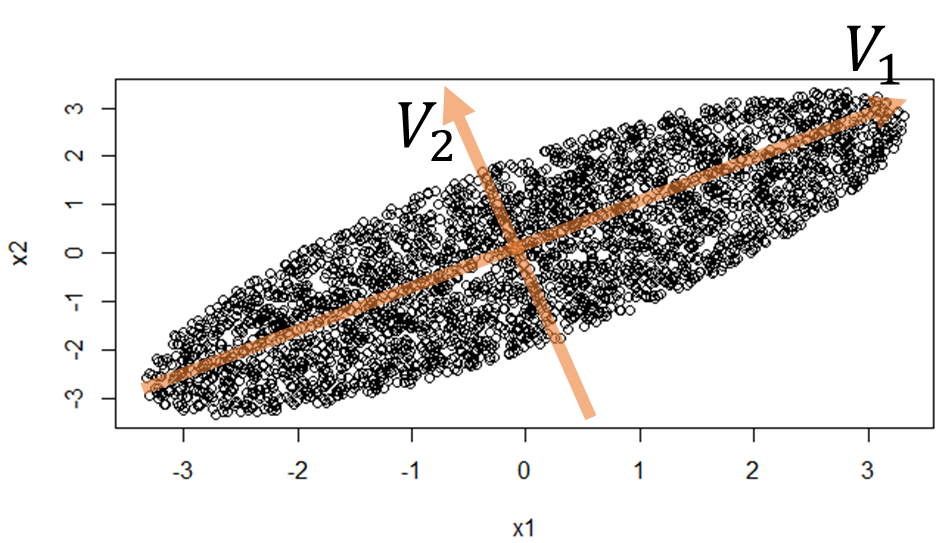
\includegraphics[width=\linewidth]{PCA_example.png}
    \caption{A dataset $\sampleMat$ (denoted by black points) where each variable has been centred (around 0) and scaled (to variance 1). The first principal component $\RSingVecs_1$ is the direction which explains direction of greatest variance, the second ($\RSingVecs_2$) represents the only other available direction which is orthogonal to $\RSingVecs_1$.}
    \label{fig:pca_example}
\end{figure}
\subsection{Introduction and singular value decomposition}
\label{PCA}
Principal component analysis (PCA) derives dominant patterns of variability from a random vector in a statistical field (in this case $\numInputs$-dimensional Euclidean space) \citep{Joliffe1992,storch_zwiers_1999} and forms new orthogonal axes to explain as much of the variability in the data as possible. These new orthogonal axes are called principal components. This process is done by taking an $\numSamples \times \numInputs$ ($\numSamples$ is the number of data points, $\numInputs$ is the number of variables) sized dataset $\sampleMat$ where each column has been centred (to mean $0$) and scaled (to variance $1$) and then determining the direction of greatest variance, which is denoted $\basis_1$; the first singular vector. Then $\basis_2$ is determined, this finds the direction of greatest variance under the condition $\basis_2 \perp \basis_1$. Then $\basis_3$ finds the greatest direction such that $\basis_3 \perp (\basis_2 \perp \basis_1)$. This continues for all $i=1\dots \matRank$ where $\matRank \leq \min(\numDPs,\numInputs)$ is the rank of the dataset $\sampleMat$.\\\\
One can find the proportion of variance explained by each singular vector $\basis_i$ by calculating 
\begin{equation}
    \label{prop_expl}
    \varExpl_i = \frac{\singVal_i^2}{\sum_{j=1}^\matRank \singVal^2},
\end{equation}
where $\singVal_i^2$ is the variance of the data along the axis $\basis_i$.\\\\
This process of selecting all $\basis_i$s to find the directions of greatest variance of $\sampleMat$ is equivalent to determining the singular value decomposition (SVD) of $\sampleMat$:
\begin{align}
    & \sampleMat = \underset{\numDPs \times \matRank}{\LSingVecs} \ \underset{\matRank \times \matRank}{\singValMat} \ \underset{\matRank \times \numInputs}{\RSingVecs^T},
    \label{SVD}
\end{align}
where $\sampleMat$ is an $\numSamples \times \numInputs$ matrix centred at $0$ with each column scaled to have variance $1$ and where $\LSingVecs$ and $\RSingVecs$ are left and right singular (and orthogonal) vectors for $\sampleMat$ respectively. This orthogonality means
\begin{align}
    & \LSingVecs^T \LSingVecs = I_\matRank \label{SVD:cond1}, \\
    & \RSingVecs^T \RSingVecs = I_\matRank \label{SVD:cond2},
\end{align}
where $\RSingVecs$ is a $\numInputs \times \matRank$ matrix containing all the singular vectors $\RSingVecs_i$ for $i=1\dots \matRank$ and $\singValMat$ is the $\matRank \times \matRank$ diagonal matrix where the square of each singular value $\singVal_i$ on the diagonal describes the proportion of variance explained by singular vector $\RSingVecs_i$ in line with eq.\eqref{prop_expl}. This process is illustrated in figure \ref{fig:pca_example}.\\\\
The SVD of $\sampleMat$ can be determined by first calculating $\singValMat$ and $\RSingVecs$ and rearranging eq.\eqref{SVD} to obtain $\LSingVecs$. By calculating $\sampleMat^T\sampleMat$:
%can be determined by calculating $\Sigma$ and $V$ (then rearranging eq.\eqref{SVD} to get $U$). This is done by computing the eigenvalues of $A^T A$ which will determine $\Sigma$ and $V$:%. Performing this calculation and using condition (\ref{SVD:cond1}) we obtain
\begin{equation}
\label{eqn:A'A}
    \sampleMat^T \sampleMat = \RSingVecs \singValMat^T \LSingVecs^T \LSingVecs \singValMat \RSingVecs^T = \RSingVecs\singValMat^T I_k \singValMat \RSingVecs^T =  \RSingVecs \singValMat^2 \RSingVecs^T,
\end{equation}
(by applying condition \eqref{SVD:cond1}). Then applying eigen-decomposition to eq.\eqref{eqn:A'A}, gives $\RSingVecs$ and $\singValMat^2$ (and hence $\singValMat$). This can also be done by computing $\sampleMat \sampleMat^T$ (where $\sampleMat \sampleMat^T = \LSingVecs\singValMat^2 \LSingVecs^T$) however $\sampleMat^T \sampleMat$ is $\numInputs\times \numInputs$ and $\sampleMat \sampleMat^T$ is $\numSamples \times \numSamples$ so the latter leads to much larger calculations for the eigen-decomposition to determine $\LSingVecs$ as $\numSamples>>\numInputs$.\\\\
The co-ordinates/weights in this new basis $V$ are contained within $\LSingVecs\singValMat$ which is obtained by rearranging eq.\eqref{SVD}. After selecting the first $\matRank'(<\matRank)$ singular vectors using eq.\eqref{prop_expl}, the weights are reduced to $(\LSingVecs\singValMat)_{1:\matRank'}$ (the first $\matRank'$ columns of $\LSingVecs\singValMat$). The other singular vectors are then truncated.\\\\
A vector in the original $p$-dimensional space can be mapped onto the rotated basis using the transformation \[w(\inputVec) = \inputVec^T \basis \] with the inverse being \[w^{-1}(\inputVec') = \inputVec'\ ^T \RSingVecs^T.\]
\section{Uncertainty Quantification \& Univariate Emulation}
\label{section:emulation}
In the event that a simulator function $\simulator$ is too expensive to run, it is useful to instead represent it with a function that is computationally cheaper, namely an emulator. This is important as some analyses can take up to tens or hundreds of thousands of model runs \citep{Tripathy2016}, which if done directly on an expensive model is completely infeasible. Whilst $\simulator$ is not a random function, it can only be run at a small number of locations meaning that away from those locations the evaluation is uncertain. In a Bayesian context, that's a random function meaning that this uncertainty can be represented using a probability distribution. Mathematically, this emulator $\emulator$ is represented as a linear set of basis functions and a zero-mean random function
\begin{equation}
    \label{eq:emulator}
    \emulator(\inputVec) = \basisFuncs^T (\inputVec) \basisCoeffs + \residual(\inputVec),
\end{equation}
where $\basisFuncs (\inputVec)$ are a set of $\numBasisFuncs$ prior basis/trend functions, $\basisFuncs$ are a set of $\numBasisFuncs$ coefficients associated with those trend functions and $\residual(\inputVec)$ is a residual function between the data and the basis functions.
\subsection{Gaussian process regression}
\label{section:GPs}
A Gaussian process (GP) emulator is one option for $\residual$ in eq.\eqref{eq:emulator}. A Gaussian process is an infinite collection of random variables where any subset of these variables forms a multivariate normal distribution \citep{Currin1991}. Through the use of a Gaussian process, one can use Bayesian inference to make predictions on outputs \citep{Currin1991,OHagan2006,Kennedy2001,Oakley2002}. The GP can be defined via a mean and covariance function which can be incorporated into the form of the emulator in eq.\eqref{eq:emulator} through 
\begin{equation}
    \nonumber
    \residual(\inputVec) \sim \GP(\mathbf{0},\text{\cov}(\simulator(\inputVec),\simulator(\inputVec'))).
\end{equation}
This means the emulator $\emulator$ in eq.\eqref{eq:emulator} has prior mean $\basisFuncs (\inputVec)^T \basisCoeffs$ where the basis functions $\basisFuncs(.)$ can be chosen to be just a constant (i.e. $\basisFuncs (\inputVec) = (1)$), linear ($\basisFuncs (\inputVec) = (1,\inputVec^T)^T$), quadratic, cubic, or any functions of input variables, and where $\basisCoeffs$ are the regression coefficients. The prior covariance between two outputs $\simulator(\inputVec)$ and $\simulator(\inputVec')$ is given by
\begin{equation}
    \label{eq:cov_corr_func}
    \cov(\simulator(\inputVec),\simulator(\inputVec')) = \var \corr(\inputVec,\inputVec')
\end{equation}
where the form of the correlation function $\corr(.,.)$ is chosen such that $\corr(\inputVec,\inputVec) = 1$, $\corr(\inputVec,\inputVec')$ is close to $1$ if the distance between $\inputVec$ and $\inputVec'$ is small and low if the distance is high.\\\\
The model for $\emulator(.)$ requires the estimation of parameters $\basisCoeffs$ and $\var$ where a prior can be specified over these two variables. In many applications, a weak prior is used which takes the form
\begin{equation}
    \label{eq:weak_prior}
    \prior(\basisCoeffs,\var) \propto \SD^{-2}.
\end{equation}
\\
The emulator is trained using model runs with the output denoted \[\designOutput = \left(\simulator(\inputVec_1),\dots,\simulator(\inputVec_\numDPs)\right) = \simulator(\designInput).\] An assumption can be made using eq.\eqref{eq:weak_prior} to model the output $\designOutput$ as
\begin{equation}
    \nonumber
    \designOutput | \basisCoeffs, \var \sim N(H \basisCoeffs, \var \corrMatrix),
\end{equation}
where $H = (\basisFuncs(\inputVec_1),\dots,\basisFuncs(\inputVec_\numDPs))$ and 
\begin{equation}
    \label{eq:A}
    \corrMatrix = 
    \begin{pmatrix}
        1 & \corr(\inputVec_1,\inputVec_2) & \dots & \corr(\inputVec_1,\inputVec_\numDPs) \\
        \corr(\inputVec_2,\inputVec_1) & 1 &  & \vdots \\
        \vdots & \ & \ddots & \vdots \\
        \corr(\inputVec_\numDPs,\inputVec_1) & \dots & \dots & 1 
    \end{pmatrix}.
\end{equation}
This allows for the emulator $\emulator$ to take the following form:
\begin{equation}
\nonumber
    \emulator(.)|\basisCoeffs,\var,\designOutput \sim \GP(m^*(.),\cov^*(.,.)),
\end{equation}
where
\begin{align}
    & m^*(\inputVec) = \basisFuncs^T(\inputVec) \basisCoeffs + \mathbf{t(\inputVec)^T} \corrMatrix^{-1} (\mathbf{\designOutput} - H\mathbf{\basisCoeffs}), \label{eq:post1-mean} \\
    & \cov^*(.,.) = \var \corr^*(.,.),\nonumber \\
    & \corr^*(\inputVec,\inputVec') = \corr(\inputVec,\inputVec') - \mathbf{t(\inputVec)} \corrMatrix^{-1} \mathbf{t(\inputVec')}, \label{eq:post1-cov}\\
    & H^T = (\basisFuncs(\inputVec_1),\dots,\basisFuncs(\inputVec_\numDPs)),\nonumber \\
    & \mathbf{t(\inputVec)}^T = \left(\corr(\inputVec,\inputVec_1),\dots,\corr(\inputVec,\inputVec_\numDPs) \right) \text{ and} \nonumber\\
    & \designOutput^T = \left(\simulator(\inputVec_1),\dots,\simulator(\inputVec_\numDPs) \right). \nonumber
\end{align}
The posterior mean in eq.\eqref{eq:post1-mean} and posterior correlation in eq.\eqref{eq:post1-cov} are updated from $\basisFuncs$ and $\corr(\inputVec,\inputVec')$ respectively using the derivations outlined in \citet{Krzanowski1988}.
Now what remains is to remove the conditioning on the unknown parameters $\mathbf{\basisCoeffs}$ and $\var$. The result from integrating out $\basisCoeffs$ gives
\begin{equation}
    \nonumber
    \emulator(.) | \designOutput,\var \sim \GP(m^{**}(.),\cov^{**}(.,.))
\end{equation}
where 
\begin{align}
    & m^{**}(\inputVec) = \mathbf{\basisFuncs^T \basisCoeffsEst} + \mathbf{t(\inputVec)}^T \corrMatrix^{-1} (\designOutput - H\basisCoeffsEst),\label{eq:post2-mean} \\
    & \cov^{**}(.,.) = \var \corr^{**}(.,.),\nonumber \\
    & \corr^{**}(\inputVec,\inputVec') = \corr(\inputVec,\inputVec') - \mathbf{t(\inputVec)} \corrMatrix^{-1} \mathbf{t(\inputVec')} \label{eq:post2-cov} \\
    & + (\mathbf{\basisFuncs^T - t(\inputVec)^T}\corrMatrix^{-1}H) (H^T \corrMatrix^{-1} H)^{-1}(\mathbf{\basisFuncs(\inputVec')^T - t(\inputVec')^T}\corrMatrix^{-1}H)^T, \nonumber\\
    & H^T = (\mathbf{\basisFuncs(\inputVec_1),\dots,\basisFuncs(\inputVec_\numDPs)}),\nonumber\\
    & \mathbf{t(\inputVec)}^T = \left(\corr(\mathbf{\inputVec,\inputVec_1}),\dots,\corr(\inputVec,\inputVec_\numDPs) \right),\nonumber\\
    & \designOutput^T = \left(\simulator(\inputVec_1),\dots,\simulator(\inputVec_\numDPs) \right) \text{ and} \nonumber\\
    & \basisCoeffs = (H^T \corrMatrix^{-1} H)^{-1} H^T \corrMatrix^{-1} \designOutput. \label{eq:post2-beta}
\end{align}
Finally, integrating out $\var$ leads to the property that
\begin{equation}
    \label{eq:student t}
    \frac{\simulator(\inputVec) - m^{**}(\inputVec)}{\SDEst\sqrt{\corr^{**}(\inputVec,\inputVec')}} \sim t_{\numDPs-\numBasisFuncs}
\end{equation}
where $t_{\numDPs-\numBasisFuncs}$ is a student $t$ random variable with $\numDPs-\numBasisFuncs$ degrees of freedom and 
\begin{equation}
    \label{eq:sigma_sq_hat}
    \varEst = \frac{\designOutput^T \corrMatrix^{-1} \designOutput -\basisCoeffsEst^T (H^T \corrMatrix^{-1} H) \basisCoeffsEst}{\numDPs - \numBasisFuncs - 2}.
\end{equation}
\subsubsection{Nugget}
\label{section:nugget}
A nugget (or `jitter') is an, often small (see \citet{Andrianakis2012,Baker2020}), noise term added to the covariance matrix $\corrMatrix$ in order to improve the inversion \citep{Andrianakis2012} whilst having a small effect on the model output $\simulator(\inputVec)$ \citep{Neal1997,Andrianakis2012}.\\\\
It is incorporated into the model by adding an extra term $\nug(.)$ to eq.\eqref{eq:emulator}:
\begin{equation}
    \label{eq:emulator-nugget}
    \emulator(\inputVec) = \basisFuncs^T(\inputVec) \basisCoeffsEst + \residual(\inputVec) + \nug(\inputVec),
\end{equation}
where $\nug(\inputVec)$ is a normally distributed random variable with mean $0$ and variance $\nugVar$ at any point $\inputVec$. The covariance of $\nug(.)$ is given by
\begin{equation}
    \nonumber
    \cov(\nug(\inputVec),\nug(\inputVec')) = 
    \begin{cases}
        \nugVar, & \inputVec = \inputVec', \\
        0, & {\textit{otherwise}}.
    \end{cases}
\end{equation}
\subsubsection{Correlation functions}
The choice of covariance function (or kernel) is important as it encodes the assumptions made about the function being emulated \citep{Rasmussen_Williams_2006}. In section \ref{section:GPs} the form of the covariance function was introduced via eq.\eqref{eq:cov_corr_func}. In this section the types of correlation functions (namely $\corr(.,.)$) are outlined. Correlation functions can be defined for each input variable $\inputVal_i$ individually and combined such that
\begin{equation}
    \label{eq:kernel-product}
    \corr(\inputVec,\inputVec') = \prod_{i=1}^\numInputs \corrXi(.,.),
\end{equation}
where $\corrXi(.,.)$ represents the correlation function for variable $\inputVal_i$.\\\\
The kernels defined in this section are stationary kernels defined by $\corrXi(\inputVec,\inputVec') = g(\inputVec-\inputVec')$. Kernels of the form $\corrXi(\inputVec,\inputVec') = g(|\inputVec-\inputVec'|)$ are known as isotropic. A kernel that has the property $\corrXi(\inputVec,\inputVec') = \corrXi(\inputVec',\inputVec)$ is called symmetric implying that any isotropic kernel is symmetric \citep{Rasmussen_Williams_2006}.\\\\
One group of kernels are the family of Mat{\'e}rn kernels \citep{Matern1947} which are defined by
\begin{equation}
    \label{eq:kernel-matern}
    \corrXi(\inputVal_i,\inputVal'_i) = \frac{2^{1-\eta}}{\Gamma(\eta)} \left(\frac{\sqrt{2 \eta} |\inputVal_i - \inputVal'_i|}{\lengthscale_i} \right)^\eta K_\eta \left(\frac{\sqrt{2 \eta} |\inputVal_i - \inputVal'_i|}{\lengthscale_i} \right)
\end{equation}
where $K_\eta$ is the modified Bessel function. The Mat{\'e}rn has $\numInputs+1$ parameters: $\eta>0$ and the lengthscale for each variable $\lengthscale_i > 0$ for $i = 1,\dots,\numInputs$. This has the property of being $\floor{\eta}$ times mean-square differentiable. By setting $\eta = s + 1/2$ (where $s \in \mathbb{N}_0$) in eq.\eqref{eq:kernel-matern} the following simplification is obtained:
\begin{equation}
    \nonumber
    \corrXi(\inputVal_i,\inputVal'_i) = \exp{\left(-\frac{\sqrt{2 \eta}|\inputVal_i - \inputVal'_i|}{\lengthscale_i} \right)} \frac{\Gamma(s + 1)}{\Gamma(2s + 1)} \sum_{i=0}^s \frac{(\numInputs+i)!}{(\numInputs-i)!\ i!} \left(\frac{\sqrt{8\eta} |\inputVal_i - \inputVal'_i|}{\lengthscale_i} \right)^{s-i}.
\end{equation}
Common choices for $\eta$ are $3/2$ and $5/2$ \citep{Tripathy2016,Despotovic2020,Tuo2020} (to the point that these kernels are generally called ``Mat{\'e}rn 3/2" and ``Mat{\'e}rn 5/2"). %This kernel is useful when the simulator being emulated is not smooth so the linear or quadratic (in the cases of $\eta = 3/2$ and $5/2$ respectively) terms interpolate between the design points and prior rather than being a smoother fit.
It is a widely-used class of kernels noted for its ability to specify the smoothness of the Gaussian process through the control of the differentiability along its realisations \citep{Borovitskiy2020}.\\\\
The realisations from the squared exponential kernel are very smooth in contrast to those from the Mat{\'e}rn $3/2$ and $5/2$ as it has a form that is infinitely differentiable and is obtained from the Mat{\'e}rn by letting $\eta \rightarrow \infty$ in eq.\eqref{eq:kernel-matern} \citep{Rasmussen_Williams_2006}. The squared exponential takes the form
\begin{equation}
    \label{eq:kernel-SE}
    \corrXi(\inputVal_i,\inputVal'_i) = \exp{\left(-\frac{|\inputVal - \inputVal'_i| ^2}{2 \lengthscale_i^2} \right)},
\end{equation}
which is defined by the lengthscale parameter $\lengthscale_i$ of variable $\inputVariable_i$. This kernel has been used by \citet{OHagan2006} and \citet{Oakley2002} in emulating a simple one-dimensional function and \citet{Oakley2004} used it to demonstrate their sensitivity analysis methods on much higher dimensional functions. If the correlation function for all variables are chosen to be the squared exponential (eq.\eqref{eq:kernel-SE}), then eq.\eqref{eq:kernel-product} can be written as
\begin{equation}
    \nonumber
    \corr(\inputVec,\inputVec') = \exp{\left((\inputVec - \inputVec')^T B (\inputVec - \inputVec') \right)}
\end{equation}
where $B$ is a $\numInputs \times \numInputs$ matrix which specifies the inverse of the lengthscales on the diagonal but allows for interaction between inputs also.\\\\
There is also the power-exponential kernel \citep{Higdon2008} (also called $\gamma$-exponential in \citet{Rasmussen_Williams_2006}) given by
\begin{equation}
    \nonumber
    \corrXi(\inputVal_i,\inputVal'_i) = \exp{\left(-\left(\frac{|\inputVal - \inputVal'_i|}{\lengthscale_i}\right)^{\gamma_i} \right)},
\end{equation}
where $\lengthscale_i$ is the lengthscale for variable $\inputVariable_i$ and $0 < \gamma_i \leq 2$ but is only mean-square differentiable at $\gamma_i = 2$ (the squared exponential). This is to be used when wanting to specify the degree of smoothness in each input dimension where $\gamma_i = 2$ is smoothest and is less smooth the more $\gamma_i$ decreases \citep{Rasmussen_Williams_2006}.
\subsubsection{Estimating hyperparameters}
\label{section:hyperparameters}
Fitting the Gaussian process requires the estimation of the chosen kernel's hyperparameters $\lengthscale$ (and $\mathbf{\gamma}$ in the case of the power-exponential \citep{Kennedy2001}) which are estimated from the data $\design = (\designInput,\designOutput)$.\\\\
A common method is using maximum likelihood estimation (MLE), derived by \citet{Rasmussen_Williams_2006}(Ch 2):
\begin{equation}
    \label{eq:ARD-MLE}
    \hypEst_{\text{MLE}} = \underset{\hyp}{\text{arg max}} \log \likelihood(\designOutput|\designInput,\hyp) = \underset{\hyp}{\text{arg max}} \ -\frac{1}{2} \left(\designOutput^T \corrMatrix_{\nugSD}^{-1} \mathbf{\designOutput} + \log|\corrMatrix_\nugSD| + \numDPs \log 2\pi \right),
\end{equation}
where $\corrMatrix_\nugSD = \corrMatrix + \nugVar I_\numDPs$ and $\nugVar$ is the variance of the nugget (see section \ref{section:nugget}). This method is incorporated in the $R$ package {\it DiceKriging} \citep{DiceKriging}.\\\\
Alternatively, one can adopt a Bayesian approach by specifying priors on each of the hyperparameters $\hyp$ and using the data $\design = (\designInput,\designOutput)$ to infer the posterior distribution \citep{Higdon2004}. The point estimate of the mode of this posterior is called maximum a posteriori (MAP) estimation which is represented as
\begin{equation}
    \hypEst_{\text{MAP}} = \underset{\hyp}{\text{arg max}} \ \log \likelihood(\designOutput,\designInput,\hyp) g(\hyp),
    \label{eq:ARD-MAP}
\end{equation}
where $g(\hyp)$ is the prior over all hyperparameters and $\likelihood(\designOutput|\designInput,\hyp)$ is represented in eq.\eqref{eq:ARD-MLE}. This method is incorporated in the Python package {\it mogp} \citep{mogptk}.
\subsection{Gaussian process classification}
\label{section:GPC}
\begin{figure}
    \centering
    \begin{subfigure}{}
        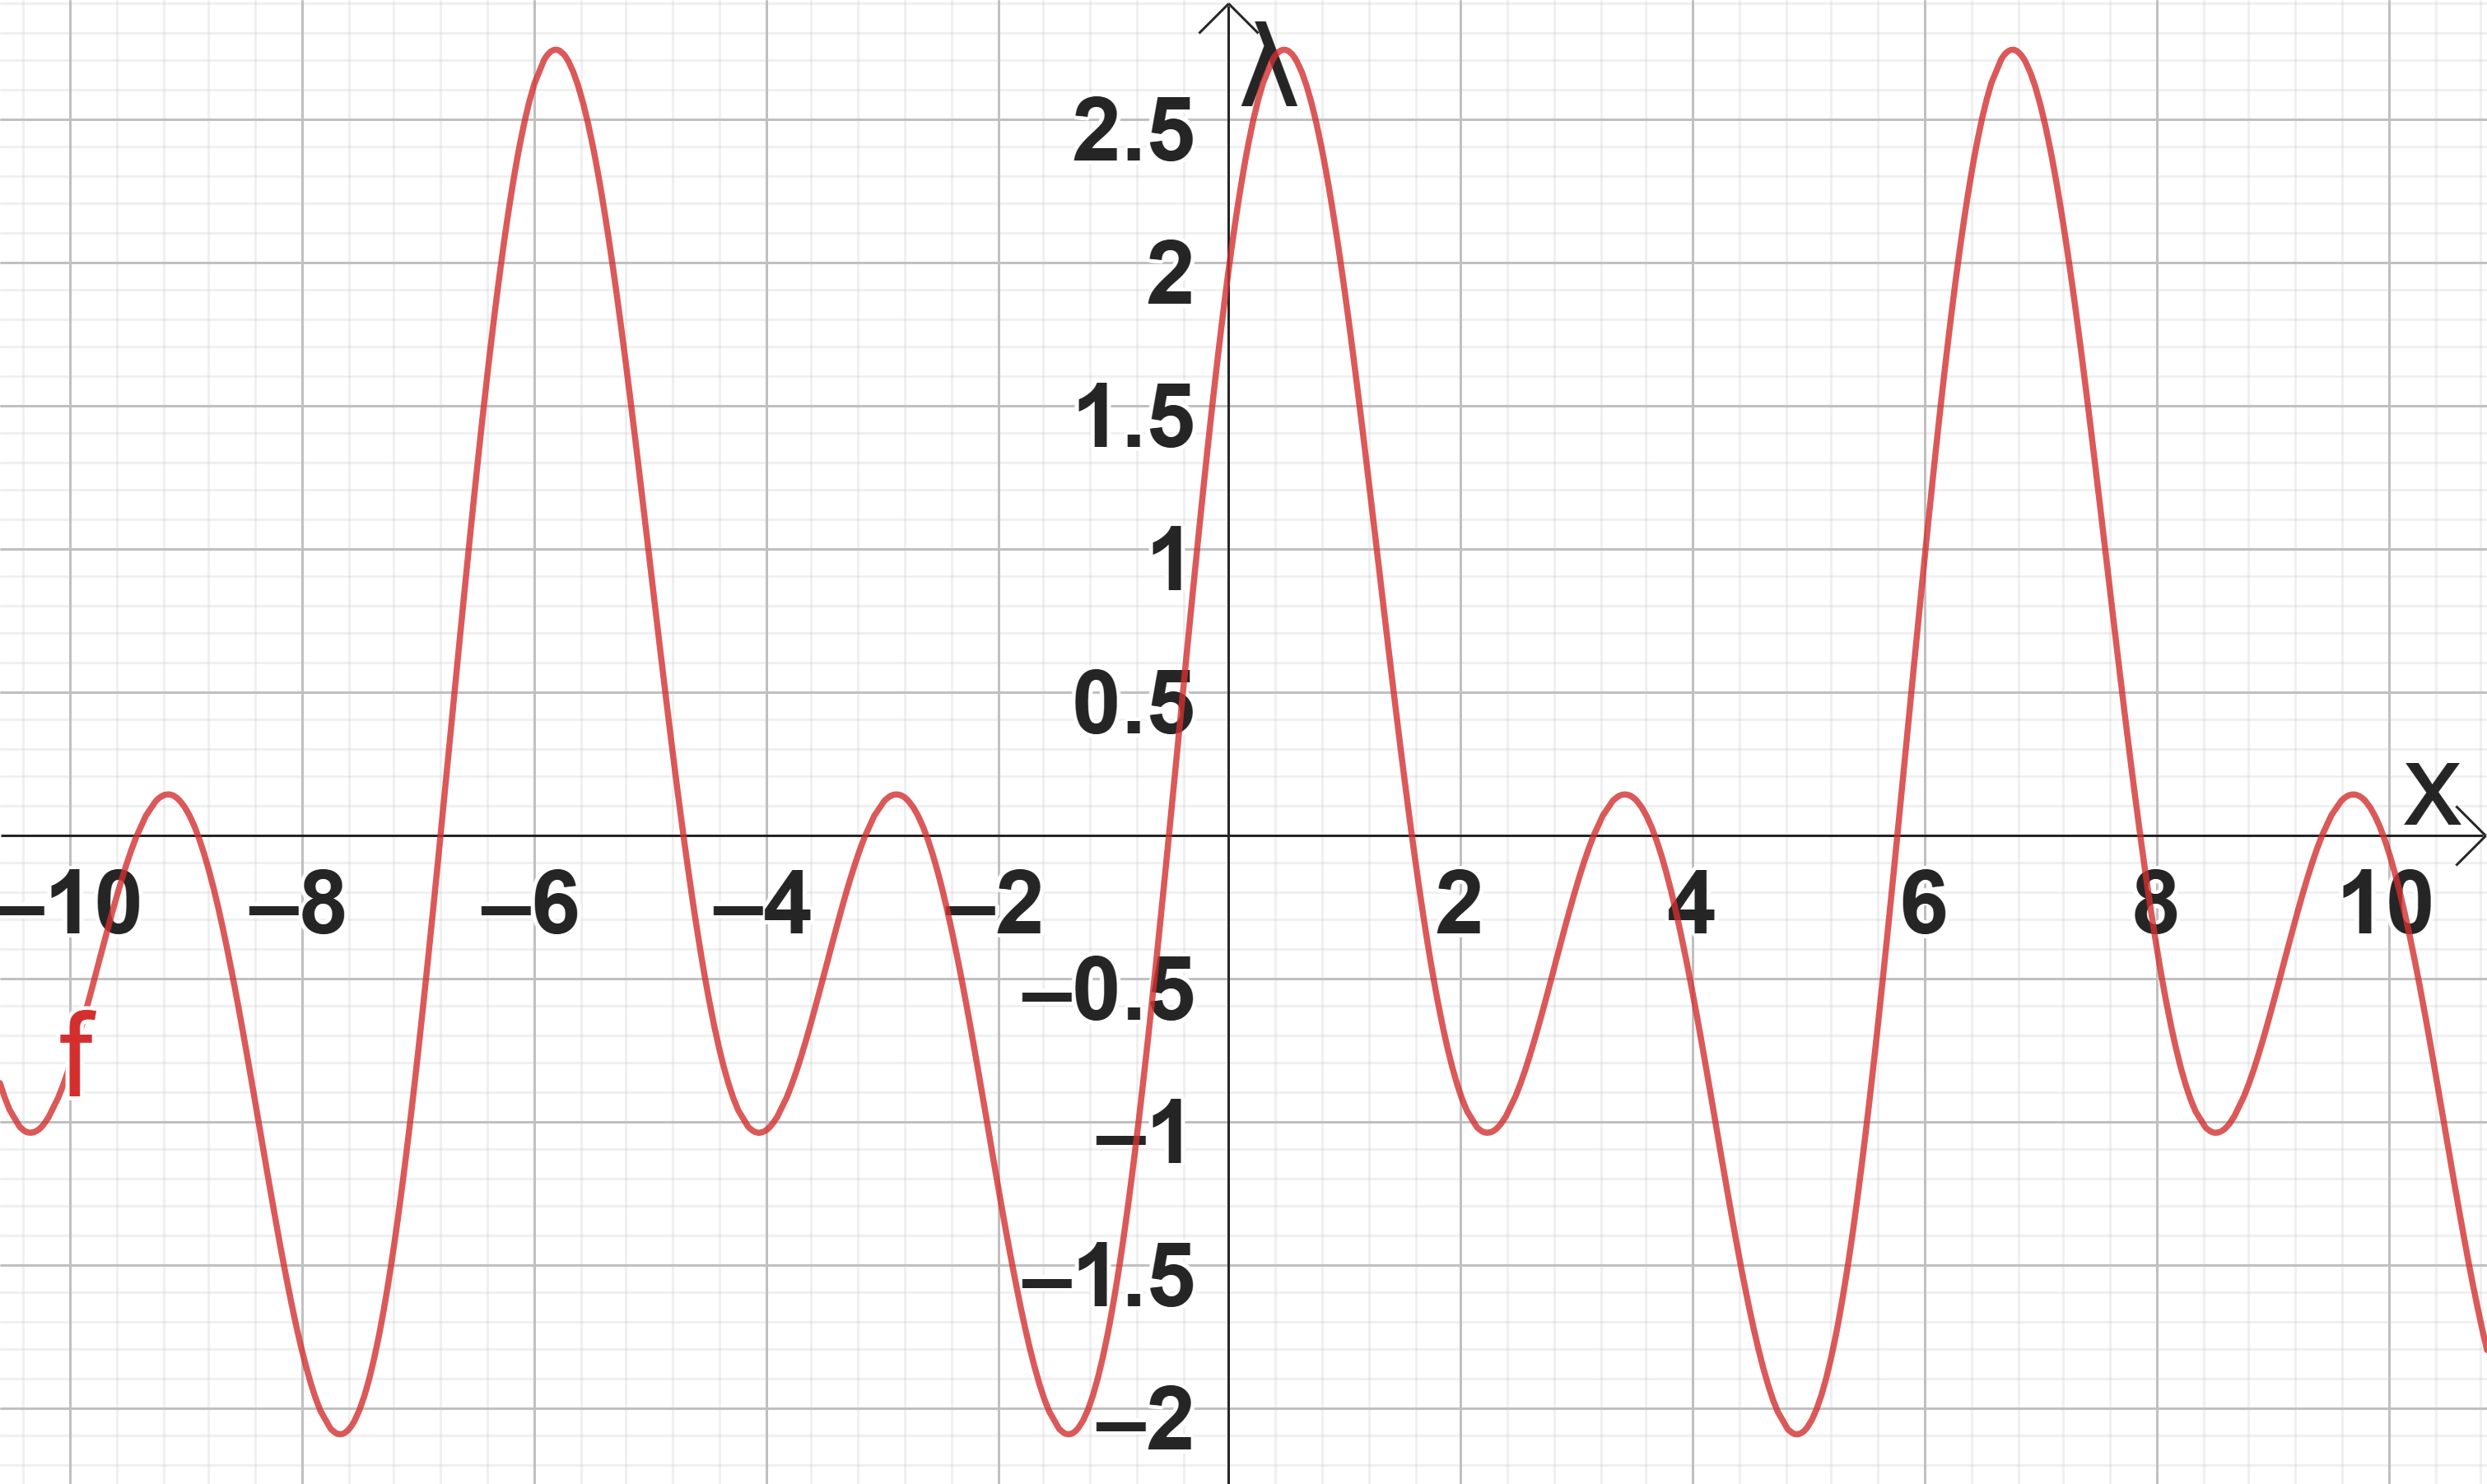
\includegraphics[width=0.45\linewidth]{GPC-explainer/latent-func.png}
        \caption{Hi}
        \label{fig:latent-func}
    \end{subfigure}
    
    \begin{subfigure}{}
        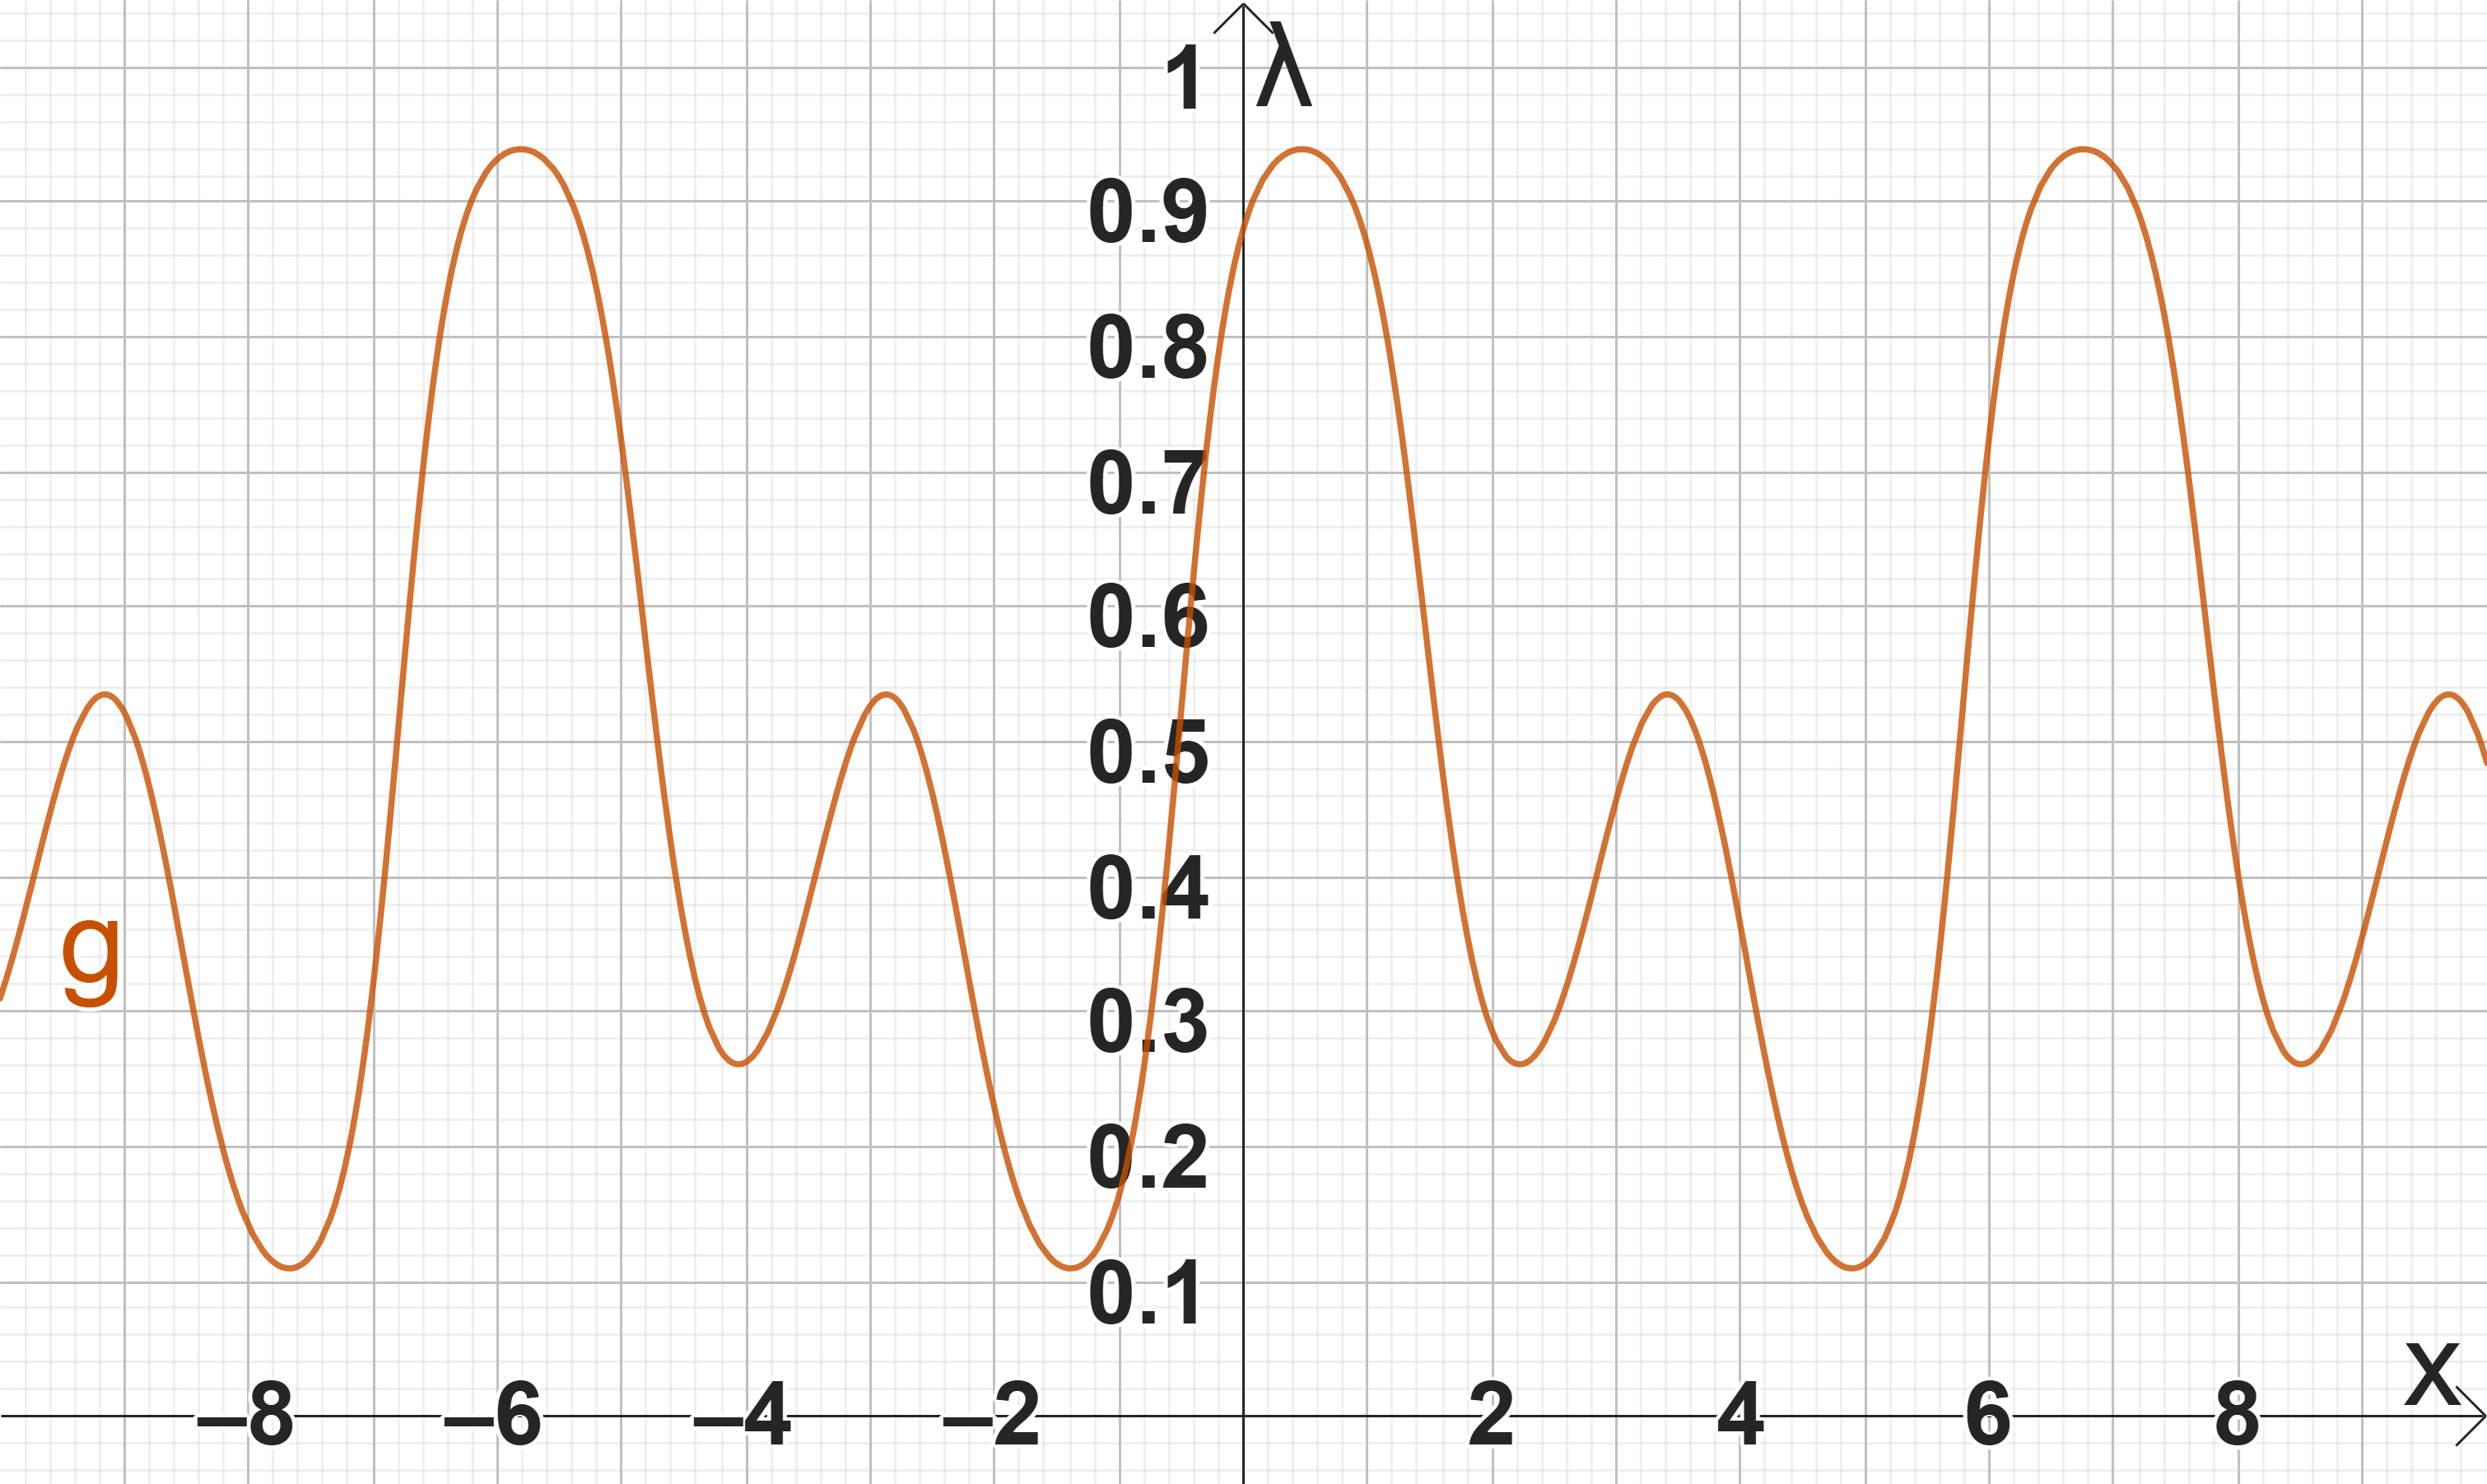
\includegraphics[width=0.45\linewidth]{GPC-explainer/posterior.png}
        \caption{Hi}
        \label{fig:posterior}
    \end{subfigure}
    \caption{Caption}
    \label{fig:GPC-explainer}
\end{figure}
A Gaussian process classifier implements a GP to make a probabilistic classification, in which test predictions take the form of class probabilities \citep{scikit-learn}. This is done using a two-step process: the first is placing a GP prior over a latent function $\latent(\inputVec)$, the second being to squish this through a logistic link function $\lambda(\inputVec)$ to obtain a probabilistic classification. In figure \ref{fig:GPC-explainer}, for a given latent function $f_*$, this is squashed through the logistic function \[\lambda(z) = \frac{1}{1+\exp(-z)}, \] i.e. figure \ref{fig:posterior} is the plot of $\lambda(f_*)$.\\\\
Calculating distribution of latent variable:
\begin{equation}
    p(f_*|\designInput,\designOutput,\inputVec_*) = \int p(f_*|\designInput,\inputVec_*,\latent) p(\latent|\designInput,\designOutput) d \latent,
\end{equation}
where $p(\latent,\designInput,\designOutput$ is posterior for latent function. Can make a probabilistic prediction using the distribution over $f_*$:
\begin{equation}
    \hat{\pi}_* \triangleq p(y_* = +1|\designInput,\designOutput,\inputVec_*) = \int \lambda(f_*) p(f_*|\designInput,\designOutput,\inputVec_*) d f_*,
\end{equation}
where $\lambda(z) = 1/(1+\exp(-z))$ is the sigmoid function.\\\\
CAN APPROXIMATE $p(\latent|\designInput,\designOutput)$ USING GAUSSIAN APPROXIMATION WHICH IS EASIER TO DEAL WITH.
\section{Multivariate emulation using PCA}
The emulation approach used in this section is the use of singular vectors obtained through principal component analysis to model the output \citep{Wilkinson_2010,Salter2019,Salter2022,Higdon2008,Sexton2012}. After an ensemble of $\numDPs$ model runs, the outputs can be represented in a $\numDPs \times \numOutputs$ matrix $\outputMat$, where $\numOutputs$ is the number of outputs. In line with the procedure behind singular value decomposition (SVD) (see section \ref{PCA}), $\outputMat$ can be first centred and scaled (mean $0$, variance $1$), then decomposed in the following way:
\begin{equation}
    \nonumber
    \outputMat = \underset{\numDPs \times \numDPs}{\LSingVecs} \ \underset{\numDPs \times \matRank}{\singValMat} \ \underset{\matRank \times \numOutputs}{\RSingVecs^T},
\end{equation}
where $\matRank = rank(\outputMat) \leq min(\numDPs,\numOutputs)$, $\singValMat$ is a diagonal matrix consisting of singular values, $\RSingVecs$ are a set of singular vectors which form the rotation and $\LSingVecs \singValMat$ are the weights where in each row $i$, this represents the mapping of co-ordinates of output space onto the new basis for the $i$th row of $\outputMat$.\\\\
Looking at $\singValMat$, one can determine the proportion of variability in the data explained by each singular value by calculating,
\begin{equation}
    \label{eqn:var_expl}
    \varExpl_i = \frac{\singVal_i^2}{\sum_{j=1}^\matRank \singVal_j^2},
\end{equation}
where $\singValMat_{i,i} = \singVal_i$. From this one can select the first $\matRank'$ singular vectors which reach a threshold $\thresh_{var}$ of variance explainability and truncate the remaining $(\matRank'+1),\dots,\matRank$ singular vectors. This can be easily calculated by setting $\matRank'$ to be the smallest value such that \[\sum_{i=1}^{\matRank'} \varExpl_i > \thresh_{var}.\]
The emulation of these $\matRank'$ principal components can be represented by
\begin{align}
    E\left[\mathbf{\emulator}(\inputVec)\right] &= \left(E\left[\emulator_1(\inputVec)\right],\dots,E\left[\emulator_{\matRank'}(\inputVec)\right] \right)^T, \label{eqn:kdim_mean} \\
    \text{Var}\left[\mathbf{\emulator}(\inputVec)\right] &= \text{diag}\left(\text{Var}\left[\emulator_1(\inputVec)\right],\dots,\text{Var}\left[\emulator_{k'}(\inputVec)\right] \right). \label{eqn:kdim_var}
\end{align}
Note that both eq.\eqref{eqn:kdim_mean}-\eqref{eqn:kdim_var} are in $\matRank'$-dimensional space. To represent them in the original $\numOutputs$-dimensional space, one simply rotates back using the first $\matRank'$ columns of $\RSingVecs$.
\begin{align}
    \overset{\numOutputs \times 1}{E\left[\mathbf{\emulator}^*(\inputVec) \right] \strut}&= \overset{\numOutputs \times \matRank'}{\RSingVecs_{1:\matRank'}\strut} \ \overset{\matRank' \times 1}{E\left[\mathbf{\emulator}(\inputVec)\right] \strut},\label{eqn:qdim_mean}\\
    \underset{\numOutputs \times \numOutputs}{\text{Var}\left[\mathbf{\emulator}^*(\inputVec) \right]\strut} &= \underset{\numOutputs \times \matRank'}{\RSingVecs_{1:\matRank'}\strut} \ \underset{\matRank' \times \matRank'}{\text{Var}\left[\mathbf{\emulator}(\inputVec)\right]\strut} \ \underset{\matRank' \times \numOutputs}{\RSingVecs_{1:\matRank'}^T\strut} + \underset{\numOutputs \times (\matRank-\matRank')}{\RSingVecs_{-1:\matRank'}\strut} \ \underset{(\matRank-\matRank')\times(\matRank-\matRank')}{\singValMat_{-1:\matRank'}\strut} \ \underset{(\matRank-\matRank') \times \numOutputs}{\RSingVecs_{-1:\matRank'}^T\strut}, \label{eqn:qdim_var}
\end{align}
where $\mathbf{\emulator}^*(\inputVec)$ is the emulator representing the full $\numOutputs$-dimensional output. By inverting the scaling and centring of $E\left[\mathbf{\emulator}^*(\inputVec) \right]$ and Var$\left[\mathbf{\emulator}^*(\inputVec) \right]$, one obtains the emulator mean and uncertainty in the original output space.\\\\
Eq.\eqref{eqn:qdim_mean} shows how the mean estimate in the full $\numOutputs$-dimensional output is represented in the much smaller $\matRank'$ dimensions as the discarded singular vectors ($\matRank-\matRank'$ of them) are modelled as noise with zero-mean. Eq.\eqref{eqn:qdim_var} shows how the variability from these discarded singular vectors (term 2) can be combined with the uncertainty arising from the emulators representing singular vectors $1,\dots,\matRank'$ (term 1).\\\\
Emulation using singular vectors provides several advantages over emulating all outputs individually:
\begin{enumerate}
    \item the dramatic reduction in the number of outputs that need to be considered, in that a smaller number of emulators are required if one where to attempt to emulate each output separately;

    \item these new outputs live on a new orthogonal basis $\basis$, meaning each principal component can be modelled independently using a GP \citep{Higdon2008} without the need for inferring correlations between them;

    \item lastly any history matching that is conducted on a $\numOutputs$-sized output results in the inversion of a $\numOutputs \times \numOutputs$ matrix each time the implausibility is calculated however \citet{Salter2022} show that this implausibility can be calculated in $\matRank' << \numOutputs$ dimensions while still accounting for the full uncertainty in $\numOutputs$ dimensions.
\end{enumerate}
The next section describes history matching and how it is done with one dimensional and $\numOutputs$-dimensional outputs using singular vectors.
\section{History Matching}
\label{section:hm}
\subsection{Introduction}
History matching is a procedure for identifying a collection of points for which the evaluation gives an acceptable match to an observation $\obs$ \citep{Vernon2010}. Before this method, the determination of an acceptable match for $\obs$ was done through trial and error by engineers running a model at random inputs, or through the use of least-squares Bayesian calibration \citep{Craig1996}. Now however, this process is simplified through the ruling out of different configurations of inputs until left with the set of points which give an acceptable match.\\\\
To compare the output of a model to the observation from reality requires accounting for two levels of uncertainty: 
\begin{enumerate}
    \item The observation $\obs$ is a measurement taken of the real-world process $\outputVec$ which therefore incurs the error induced by making this measurement. This is called {\it observation error}. This is expressed as
    \begin{equation}
        \label{eqn:obs_err}
        \outputVec = {\obs} \oplus \obsErrorqD,
    \end{equation}
    where $\obsErrorqD$ is the observation error \citep{Bower2010}.

    \item There is also an error induced by modelling the real world process $\outputVec$ using the model $\simulator$ evaluated at the `perfect input' $\inputVec^*$, which is called {\it model discrepancy}. This is expressed as
    \begin{equation}
        \label{eqn:model_disc}
        {\bf \outputVec = \simulator(\inputVec^*)} \oplus \modelDiscqD,
    \end{equation}
    where $\modelDiscqD$ is the model discrepancy.
\end{enumerate}
The aim of history matching is to find all possible values $\inputVec^* \in \paramSpace$ (where $\paramSpace$ represents the input parameter space) that satisfy eqns.\eqref{eqn:obs_err}-\eqref{eqn:model_disc}. In the case that output size $\numOutputs=1$, these equations can be combined to give:
\begin{equation}
    \label{eqn:impl-true}
    E\left[(\obs - \simulator(\inputVec^*))^2 \right] = Var[\obsError] + Var[\modelDisc].
\end{equation}
Given the expensive nature of the model, evaluating $\simulator$ to find $\inputVec^*$ is not feasible, therefore an emulator $\emulator$ can be used to approximate $\simulator$. For a given $\inputVec$, $\emulator(\inputVec)$ gives both a mean and variance therefore changing eqn.\eqref{eqn:impl-true} to
\begin{equation}
    \label{eqn:impl-approx}
    \left(\obs - E\left[\emulator(\inputVec^*)\right]\right)^2 = Var\left[\emulator(\inputVec^*)\right] + Var[\obsError] + Var[\modelDisc].
\end{equation}
By comparing the ratio of the left-hand side to the right-hand side of eq.\eqref{eqn:impl-approx}, this leads to a computationally cheap way to assess how implausible a given input $\inputVec$ is. This ratio is just the centring and scaling using the posterior mean and covariance of $\emulator(\inputVec)$ (such that the standard deviation is $1$); then assessing where the observation $\obs$ sits within this scaled posterior. This ratio is called the {\it implausibility measure}:
\begin{equation}
    \nonumber
    \impl^2(\inputVec) = \frac{\left(\obs - E\left[\emulator(\inputVec^*)\right]\right)^2}{Var\left[\emulator(\inputVec^*)\right] + Var[\obsError] + Var[\modelDisc]},
\end{equation}
where $\impl$ denotes implausibility, with the higher implausibility implying a higher chance of a point $\inputVec$ being more unlikely for $\simulator(\inputVec)$ to be close to $\obs$. 
This therefore involves establishing a threshold $\thresh$ by which $\impl(.)$ must be less than for any point $\inputVec$ not to be deemed implausible given $\obs$:
\begin{equation}
    \label{eqn:threshold}
    \NROYspace = \{\inputVec \in \paramSpace: \impl(\inputVec)<\thresh\},
\end{equation}
where $\paramSpace$ represents the whole input parameter space.
Many papers \citep{Craig1997,Vernon2010,Iskauskas2022,Williamson2017} use a result from \citet{Pukelsheim1994} which states that any univariate and unimodel distribution has 95\% of the data in at most $\pm 3\SD$ from the mean. For this reason $\thresh=3$ is widely used as the threshold.\\\\
The form of the implausibility $\impl(.)$ in eq.\eqref{eqn:impl} is only for the case that $\numOutputs=1$.\\\\
One can use an alternative measure for implausibility for multi-dimensional output that can allow for correlated outputs, errors and discrepancies:
\begin{equation}
    \label{eqn:impl}
    \impl^2(\inputVec) = \left(\obsqD - E\left[\mathbf{\emulator}(\inputVec)\right]\right)^T \left(Var\left[\mathbf{\emulator}(\inputVec)\right] + Var[\obsErrorqD] + Var[\modelDiscqD] \right)^{-1} \left(\obsqD - E\left[\mathbf{\emulator}(\inputVec)\right]\right),
\end{equation}
where the variance term on right-hand side (middle) is a $\numOutputs \times \numOutputs$ matrix to be inverted. This is equivalent to computing the Mahalanobis distance between the observation $\obsqD$ and an input to $\mathbf{\emulator}(.)$. In this case, the choice of $\thresh=3$ is no longer appropriate given the higher dimensions. A commonly used threshold is $\thresh^2=\NROYspace_{\numOutputs,0.995}^2$, which represents the 99.5th percentile of the Chi-squared distribution with $\numOutputs$ degrees of freedom \citep{Vernon2010,Andrianakis2015,Salter2019}. Often it is difficult to specify the full correlation structure for $Var[\obsErrorqD]$ and $Var[\modelDiscqD]$ so it is often assumed that these errors are uncorrelated so the matrices are diagonal \citep{Andrianakis2015}.
\subsection{The algorithm}
\label{section:hm-algorithm}
History matching is performed in iterations (commonly called waves). The process starts with the whole input space designated as NROY (not ruled out yet) space. A design is then sampled from this space, suitable emulators are built and using an implausibility measure, some input configurations are ruled out thereby defining a new NROY space. This process then repeats until either NROY is the empty set or no more space can be ruled out due to prescribed errors and discrepancies.\\\\
%{\it Brief discussion about how history matching algorithms have changed.}\\\\
\citet{Craig1996,Craig1997} were the first to establish a detailed algorithm for history matching. They address the need for elicitation of both model discrepancy and observation error, alongside any prior means or covariances for $\outputVec$. From there, \citet{Vernon2010,Vernon2014,Andrianakis2015} (and many others since) have used a consistent algorithm though modified slightly from the original by doing ensembles of model runs instead of individual runs.\\\\
The following algorithm is consistent with the recently defined procedures. It details the tradidional history matching process:
\begin{enumerate}
    \item \label{section:hm-setup} Identify target outputs $\obsqD$, model discrepancy $\modelDiscqD$ and observation error $\obsErrorqD$ using elicitation from model experts/engineers. Choose ranges for each input variable. Construct space filling design $\design_1$. Set wave number $j=1$ and wave 0 NROY space $\NROYspace_0 = \paramSpace$.

    \item Build emulators $\mathbf{\emulator}(\inputVec)$.

    \item Calculate implausibility (eq.\eqref{eqn:impl}) $\impl_j(\inputVec)$ using $\obsqD,\modelDiscqD,\obsErrorqD$ and emulators $\mathbf{\emulator}(\inputVec)$. Set $\NROYspace_j = \{\inputVec \in \paramSpace:\impl_1(\inputVec),\dots,\impl_j(\inputVec)<\thresh\}$.

    \item \label{section:hm-refocus} Sample in the space $\NROYspace_j$ to obtain design $\design_{j+1}$.

    \item If (a) $Var\left[\mathbf{\emulator}\right]<<Var[\modelDiscqD]+Var[\obsErrorqD]$ OR (b) $\NROYspace_j = \emptyset$, proceed to step \ref{alg:hm_alt-end}. Else return to step 1 and set $j=j+1$.

    \item \label{alg:hm_alt-end} If (a) then sample from $\NROYspace_j$ to obtain inputs close to target output. If (b) then restart process with higher model discrepancy or observation error.
\end{enumerate} 
\subsection{Specifying model discrepancy and observation error}
Stage \ref{section:hm-setup} of the history matching process involves the setup of the procedure. Part of this stage involves choosing the model discrepancy $\modelDiscqD$ and observation error $\obsErrorqD$. This involves consulting and eliciting from model experts the values for these two terms. These discrepancies between the simulator and reality can be difficult to incorporate into the analysis \citep{Craig1996}.\\\\
In the case of one output ($\numOutputs=1$), this only requires the specification of one variance each for $\obsErrorqD$ and $\modelDiscqD$. In \citet{Dunne2022} the model discrepancy variance was chosen through the assumption that the model predicts the output to be within $\pm 20\%$ of the observation $95\%$ of the time. This was done through consultation with the model developer.\\\\
For higher $\numOutputs$, this requires the specification of a $\numOutputs \times \numOutputs$ sized matrix for both model discrepancy and observation error. In the case of these errors being uncorrelated (i.e. error in one of the outputs of a model doesn't affect another), then these matrices are diagonal; vastly reducing the elicitation required from experts. In \citet{Craig1997} for instance, the engineer was satisfied that the observation error could be modelled as uncorrelated; therefore only requiring $\numOutputs=77$ specifications.\\\\
In the case of correlated errors however, this requires the specification of the full $\numOutputs \times \numOutputs$ matrix for both observation error and model discrepancy which leads to obvious elicitation difficulties.
\subsection{History matching using singular vectors}
\label{hm-singVec}
To incorporate the use of singular vectors in the emulation process, replace step 2 of history matching algorithm with the following sub-steps:
\begin{enumerate}
    \item[a] Take the design output $\outputMat$ ($\numDPs \times \numOutputs$) from the design $\design_j$, centre (to 0) and scale (to variance 1) and apply the singular value decomposition.

    \item[b] Map the design output $\outputMat$ onto new basis: $\outputMat' = \outputMat \RSingVecs$.

    \item[c] Select first $\matRank'$ columns of $\outputMat'$ according to eq.\eqref{eqn:var_expl}.
    
    \item[d] Construct $\matRank'$ emulators $\mathbf{\emulator^*}(\inputVec)$, where the $i$th emulator is trained by the inputs $\designInput$ and the outputs being the $i$th column of $\outputMat'$. These emulators take the form of eqs.\eqref{eqn:kdim_mean} \& \eqref{eqn:qdim_var}.
    
    \item[e] Use eqs.\eqref{eqn:qdim_mean} \& \eqref{eqn:qdim_var} to represent the full $\numOutputs$-dimensional output. Finally, reverse the scaling and centring.
\end{enumerate}
%In the previous section, the form of the emulator to represent the full output is presented in eqs.\eqref{eqn:qdim_mean}-\eqref{eqn:qdim_var}. In this section, history matching using these singular vectors is detailed.\\\\
For a point in input space to be deemed non-implausible, it needs to satisfy $\impl(\inputVec) < \thresh$, where $\thresh$ represents the threshold. \citet{Vernon2010,Andrianakis2015,Salter2019} all use a threshold of $\thresh^2 = \chi_{\numOutputs,0.995}^2$, which is the $99.5$th percentile of the chi-squared with $\numOutputs$ degrees of freedom.\\\\
Upon construction of the emulator $\mathbf{\emulator}^*(\inputVec)$, history matching can be conducted. One may be tempted to history match in the $\matRank' \ (<< \matRank \leq \numOutputs$) dimensional subspace (to lower the implausibility threshold) however \citet{Salter2019} show how one could unintentionally rule out parts of $\numOutputs$-dimensional space consistent with $\obsqD$ when history matching this way.\\\\
%The history matching process starts with the construction of an emulator $\mathbf{\emulator}^*(.)$ and a specification of an observation $\obsqD$, model discrepancy $\modelDiscqD$ and observation error $\obsErrorqD$.
The first wave is carried out by applying eq.\eqref{eqn:impl} across the input space and applying the threshold $\thresh$ thus defining the following space \[\NROYspace_1 = \{\inputVec : \impl_1^2(\inputVec) < \thresh \},\] where $\impl_i^2$ represents eq.\eqref{eqn:impl} applied to the emulator from wave $i$.\\\\
This leaves a subspace $\NROYspace_1$ of the original which is non-implausible given the data, observation and pre-prescribed errors. This space is then sampled, emulators built and implausibility applied to define \[\NROYspace_2 = \{\inputVec: \inputVec \in \NROYspace_1, \ \impl_2^2(\inputVec) < \thresh \},\] leading to the generalisation \[\NROYspace_i = \{\inputVec: \inputVec \in \NROYspace_1,\dots,\NROYspace_{i-1}, \ \impl_i^2(\inputVec) < \thresh \}.\] History matching continues in these waves until either all space is ruled out (in which case the process restarts with a larger $\obsErrorqD$ or $\modelDiscqD$), or if the uncertainty from the emulation is much smaller than the pre-prescribed errors (signifying that the non-implausible space is almost as small as it could get).
\section{Problem}
\begin{figure}[t]
    \centering
    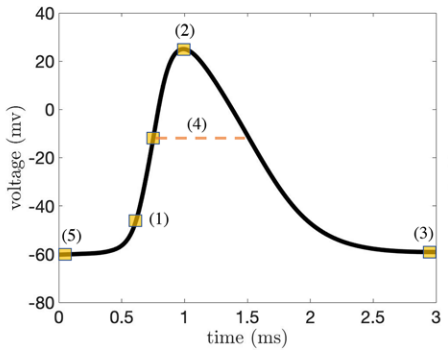
\includegraphics[width=\linewidth]{spike_characteristics.png}
    \caption{A curve describing an action potential from \citet{Saghafi2024}. This example is characterised in 5 ways: (1): action potential threshold, (2): action potential peak; (3): action potential trough; (4): action potential width and (5): action potential minimum before pulse.}
    \label{fig:spike_char}
\end{figure}
Have real-world data and want to find parameter values which give suitable match to this data when evaluated by model. The real-world data can be broken down into characteristics (see figure \ref{fig:spike_char}). The problem is therefore that we have a simulator $\outputVec = \mathbf{\simulator}(\inputVec)$, where $\outputVec = \{\outputVec_{class}, \outputVec_{char}\}$ contains the classification of whether a spike is induced at $\inputVec$ (either 0,1) and what characteristics the spike has if it is induced respectively. \\\\
The problem is to find suitable parameter values which when evaluated by $\mathbf{\simulator}$ give characteristics close to the real-world data.
\section{Framework to solve problem}
The problems in this process are two-fold: one is the areas of input space that result in a spike, and the second is the characteristics of that spike conditional on if it occurs. In this report, these problems are treated separately; first a Gaussian process classifier is constructed to divide the parameter space into two regions (spike (1) and not spike (0)), and second, within the spike space, the characteristics of that spike is emulated using Gaussian process emulators.
\subsection{Classification problem}
\label{method-class}
A Latin hypercube design \citep{lhs} is used to sample across parameter space. The output of this design is either a 1 (spike) or 0 (no spike). A Gaussian process classifier (see section \ref{section:GPC}) is constructed using this training data with the domain over the parameter space. Therefore, at a given point in this parameter space, a probability is given of a spike being induced.\\\\
The initial design is uniform, however in practise it is likely that different regions of parameter space require a higher concentration of points to clearly establish the boundary between spiking and not spiking regions. Because of this, there are likely to be many points close to the boundary of 0.5 (probability of spiking), therefore further samples are taken whose probabilities are close to this value. This has the effect of pushing the probabilities across the parameter space towards 1 and 0 enabling a more reliable prediction.\\\\
Several iterations of this can be done, more clearly establishing the boundary between spiking and not spiking. In practise, a check at the proportion of points close to the boundary was taken and stopping criteria was initiated when the improvement after each new iteration was small. 
\subsection{Characteristic problem}
The result from using the classifier is a region of parameter space where the probability of spiking is 0.5. A more conservative approach (to perhaps avoid misclassifying) can be used by choosing a probability lower than 0.5 or a more restrict approach by using a higher probability.\\\\
In the space that is remaining (denoted $\NROYspace_0$), the characteristics of the simulator output are emulated and history matching can be undertaken to rule out regions of parameter space deemed implausible given the model runs and target outputs.\\\\
Wave 1 is undertaken by sampling across the whole parameter space such that the probability of spiking is greater than 0.5. This is done using the methodologies established in section \ref{hm-singVec}. There are a number of characteristics that can be emulated (see figure \ref{fig:spike_char}) which therefore changes the number of outputs $\numOutputs$ and the implausibility threshold $\thresh$. The result of this history matching wave reduces the space to $\NROYspace_1$.\\\\
The next wave begins with sampling in $\NROYspace_1$, constructing emulators whose domain is in this region and once again ruling out space using the implausibility measure. This in turn gives $\NROYspace_2$. This process continues until the variance of the emulators is small compared to the pre-prescribed observation error and model discrepancy.
\section{Example 1}
\subsection{Setup}
Hodgkin-Huxley model compressed into 3 inputs: $g_{Na}, g_K, injCurrent$ with ranges $[50,300], [0,40], [0,20]$ respectively. There are 6 outputs: {\it class, maxV, minV, width, minVbp, threshold}. One model run at a random input value is used to generate the observation to history match to: i.e. $\outputVec^* = \simulator(\inputVec^*)$. For this example:\[\inputVec^* = (g_{Na}^*,g_K^*,injCurrent^*) = (163.62, 19.855, 3.0570)\] and \[\outputVec^* = (class^*, maxV^*, minV^*, width^*, minVbp^*, threshold^*)\]\[ = (1, 43.329, -54.460, 1.2300, -54.460, -47.412).\]
\subsection{Classification GP results}
\begin{figure}[t]
    \centering
    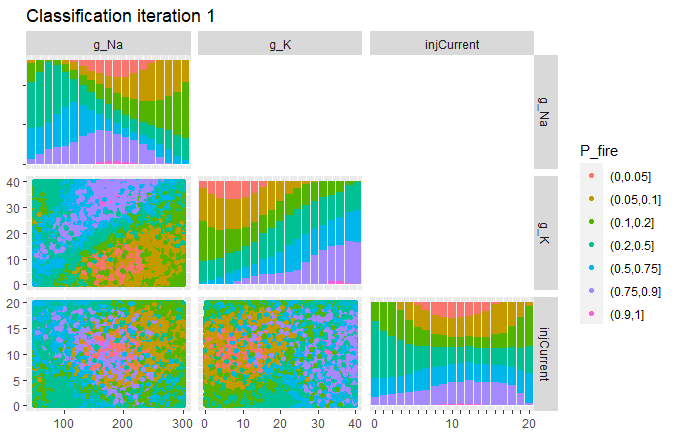
\includegraphics[width=\linewidth]{Example1/class1.png}
    \caption{Iteration 1 of the Gaussian process classifier. The diagonal shows the probabilities across the marginal of each variable. The lower triangle shows the probabilities across each of the two-dimensional windows. The different colours represent probabilities which are sorted into bins listed to the right of the plot.}
    \label{fig:ex1-class1}
\end{figure}

\begin{figure}[t]
    \centering
    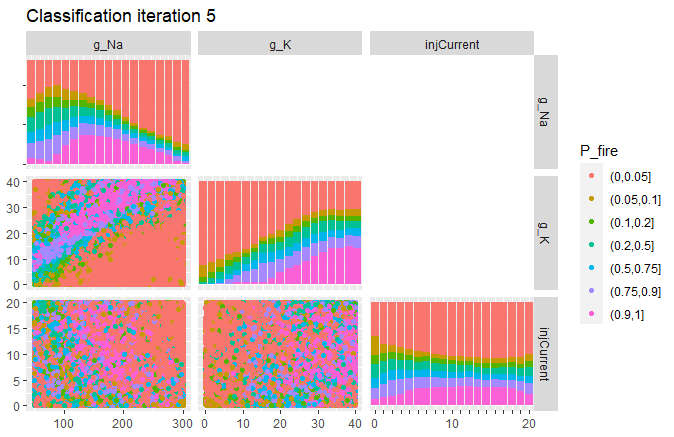
\includegraphics[width=\linewidth]{Example1/class5.png}
    \caption{Iteration 5 of the Gaussian process classifier. The diagonal shows the probabilities across the marginal of each variable. The lower triangle shows the probabilities across each of the two-dimensional windows. The different colours represent probabilities which are sorted into bins listed to the right of the plot.}
    \label{fig:ex1-class5}
\end{figure}
Applying the methodology in section \ref{method-class} for one iteration yields figure \ref{fig:ex1-class1}. Looking at the diagonal plot, one sees the proportion of parameter space which lies in the different probability bins. Much of the probabilities in the parameter space are between 0.2 and 0.75. Sampling from this space again starts to separate out these regions and move points away from the boundary.\\\\
By iteration 5, far more of these probabilities have moved away from the 0.5 boundary and pushed towards 0 and 1. Looking at the off-diagonal plots show how these different probabilities show the boundaries between firing and not firing.\\\\ After this point, the improvement in each new iteration was negligible therefore this was chosen to be the final iteration. Therefore the space remaining is defined as \[\NROYspace_0 = \{\inputVec:P(\inputVec=fire)>0.5 \}.\] This space is plotted in figure \ref{fig:ex1-char0}.
\subsection{Characteristic GP results}
\begin{figure}[t]
    \centering
    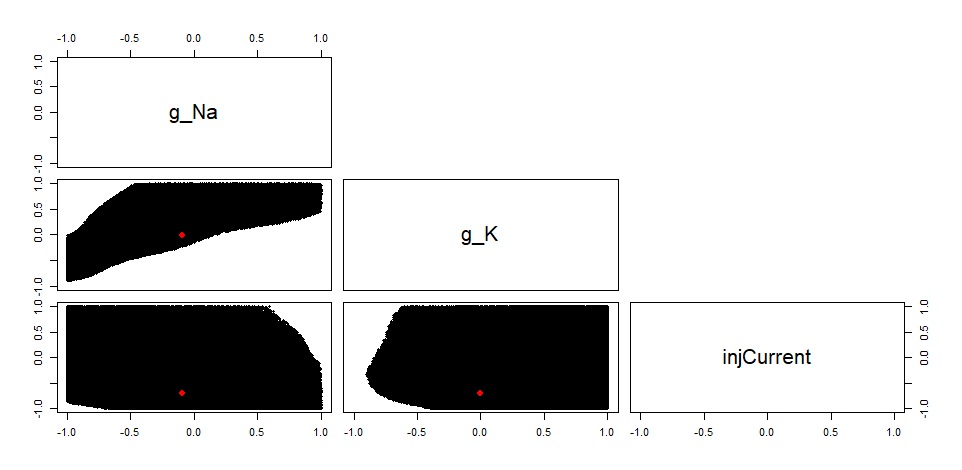
\includegraphics[width=\linewidth]{Example1/char0.png}
    \caption{NROY space after using Gaussian process classifier. The red dot is $\inputVec^*$. All inputs have been scaled to $[-1,1]^p$.}
    \label{fig:ex1-char0}
\end{figure}
\begin{figure}
    \centering
    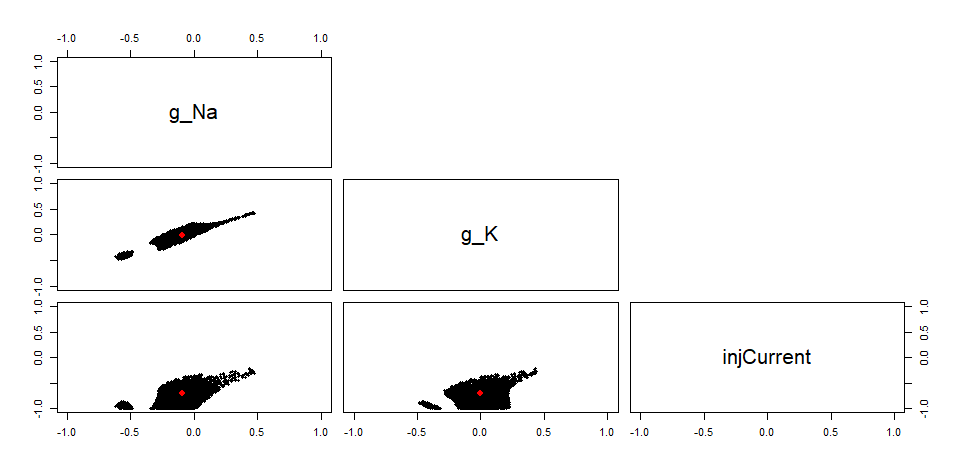
\includegraphics[width=\linewidth]{Example1/char1.png}
    \caption{NROY space after 1 wave of history matching. The red dot is $\inputVec^*$. All inputs have been scaled to $[-1,1]^p$.}
    \label{fig:ex1-char1}
\end{figure}
\begin{figure}[t]
    \centering
    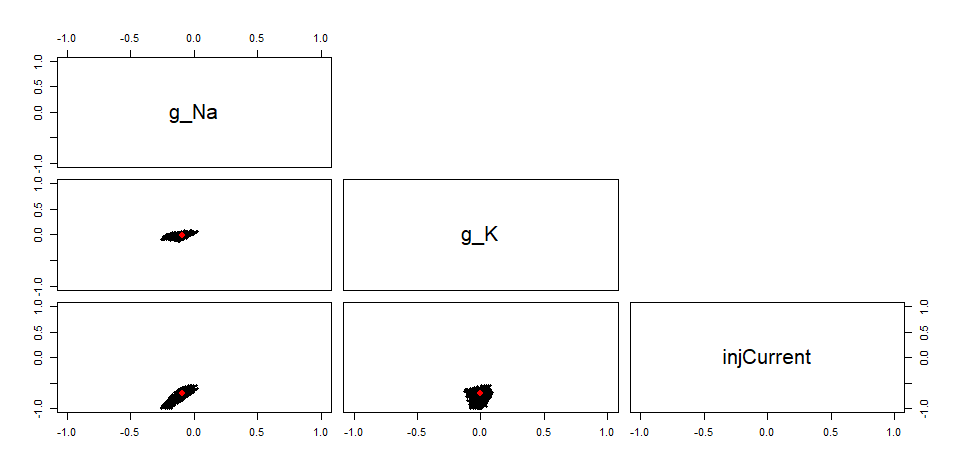
\includegraphics[width=\linewidth]{Example1/char2.png}
    \caption{NROY space after 2 waves of history matching. The red dot is $\inputVec^*$. All inputs have been scaled to $[-1,1]^p$.}
    \label{fig:ex1-char2}
\end{figure}
\begin{figure}[t]
    \centering
    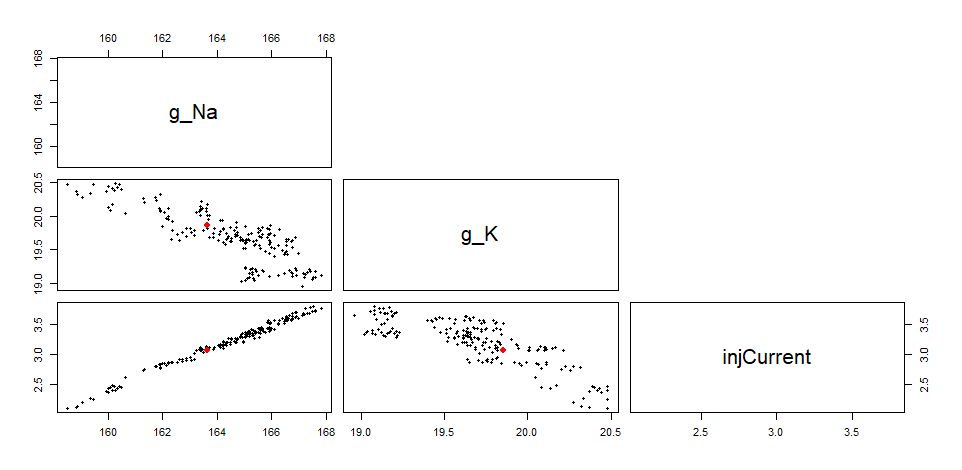
\includegraphics[width=\linewidth]{Example1/char15_zoomed_orig.png}
    \caption{NROY space after 15 waves of history matching, zoomed in. The red dot is $\inputVec^*$.}
    \label{fig:ex1-char15_zoomed}
\end{figure}
Now remains the history matching procedure where the target output is $\outputVec^*$. In practise, an observation error variance and model discrepancy variance would also be specified but as this example serves as a demonstration of the methods, instead these have been set to $10^{-6}$ for each output.\\\\
History matching will be done over the space defined by $\NROYspace_0$. This space is sampled, evaluated by the emulator and thus able to define a new set $\NROYspace_1$. After one wave of history matching, figure \ref{fig:ex1-char1} shows the space remaining and figure \ref{fig:ex1-char2} shows the space contained in $\NROYspace_2$.\\\\
This continued until wave 15, in which approximately 1/5 millionth of the original parameter space remains. The zoomed in plot of $\NROYspace_15$ is shown in figure \ref{fig:ex1-char15_zoomed} with the input values scaled back to their true scales. Using the points contained in this plot, the emulator can be evaluated and a prediction made as to what $\outputVec^*$ is. WHAT WAS THIS GUESS?
\newpage
\bibliographystyle{agsm}
\bibliography{references.bib}
\end{document}
